\documentclass[a4paper,12pt,twoside]{memoir}

% Castellano
\usepackage[spanish,es-tabla]{babel}
\selectlanguage{spanish}
\usepackage[utf8]{inputenc}
\usepackage[T1]{fontenc}
\usepackage{lmodern} % scalable font
\usepackage{microtype}
\usepackage{placeins}

\RequirePackage{booktabs}
\RequirePackage[table]{xcolor}
\RequirePackage{xtab}
\RequirePackage{multirow}

% Links
\usepackage[colorlinks]{hyperref}
\hypersetup{
	allcolors = {red}
}

% Ecuaciones
\usepackage{amsmath}

% Rutas de fichero / paquete
\newcommand{\ruta}[1]{{\sffamily #1}}

% Párrafos
\nonzeroparskip


% Imagenes
\usepackage{graphicx}
\newcommand{\imagen}[2]{
	\begin{figure}[!h]
		\centering
		\includegraphics[width=0.9\textwidth]{#1}
		\caption{#2}\label{fig:#1}
	\end{figure}
	\FloatBarrier
}

\newcommand{\imagenflotante}[2]{
	\begin{figure}%[!h]
		\centering
		\includegraphics[width=0.9\textwidth]{#1}
		\caption{#2}\label{fig:#1}
	\end{figure}
}



% El comando \figura nos permite insertar figuras comodamente, y utilizando
% siempre el mismo formato. Los parametros son:
% 1 -> Porcentaje del ancho de página que ocupará la figura (de 0 a 1)
% 2 --> Fichero de la imagen
% 3 --> Texto a pie de imagen
% 4 --> Etiqueta (label) para referencias
% 5 --> Opciones que queramos pasarle al \includegraphics
% 6 --> Opciones de posicionamiento a pasarle a \begin{figure}
\newcommand{\figuraConPosicion}[6]{%
  \setlength{\anchoFloat}{#1\textwidth}%
  \addtolength{\anchoFloat}{-4\fboxsep}%
  \setlength{\anchoFigura}{\anchoFloat}%
  \begin{figure}[#6]
    \begin{center}%
      \Ovalbox{%
        \begin{minipage}{\anchoFloat}%
          \begin{center}%
            \includegraphics[width=\anchoFigura,#5]{#2}%
            \caption{#3}%
            \label{#4}%
          \end{center}%
        \end{minipage}
      }%
    \end{center}%
  \end{figure}%
}

%
% Comando para incluir imágenes en formato apaisado (sin marco).
\newcommand{\figuraApaisadaSinMarco}[5]{%
  \begin{figure}%
    \begin{center}%
    \includegraphics[angle=90,height=#1\textheight,#5]{#2}%
    \caption{#3}%
    \label{#4}%
    \end{center}%
  \end{figure}%
}
% Para las tablas
\newcommand{\otoprule}{\midrule [\heavyrulewidth]}
%
% Nuevo comando para tablas pequeñas (menos de una página).
\newcommand{\tablaSmall}[5]{%
 \begin{table}
  \begin{center}
   \rowcolors {2}{gray!35}{}
   \begin{tabular}{#2}
    \toprule
    #4
    \otoprule
    #5
    \bottomrule
   \end{tabular}
   \caption{#1}
   \label{tabla:#3}
  \end{center}
 \end{table}
}

%
%Para el float H de tablaSmallSinColores
\usepackage{float}

%
% Nuevo comando para tablas pequeñas (menos de una página).
\newcommand{\tablaSmallSinColores}[5]{%
 \begin{table}[H]
  \begin{center}
   \begin{tabular}{#2}
    \toprule
    #4
    \otoprule
    #5
    \bottomrule
   \end{tabular}
   \caption{#1}
   \label{tabla:#3}
  \end{center}
 \end{table}
}

\newcommand{\tablaApaisadaSmall}[5]{%
\begin{landscape}
  \begin{table}
   \begin{center}
    \rowcolors {2}{gray!35}{}
    \begin{tabular}{#2}
     \toprule
     #4
     \otoprule
     #5
     \bottomrule
    \end{tabular}
    \caption{#1}
    \label{tabla:#3}
   \end{center}
  \end{table}
\end{landscape}
}

%
% Nuevo comando para tablas grandes con cabecera y filas alternas coloreadas en gris.
\newcommand{\tabla}[6]{%
  \begin{center}
    \tablefirsthead{
      \toprule
      #5
      \otoprule
    }
    \tablehead{
      \multicolumn{#3}{l}{\small\sl continúa desde la página anterior}\\
      \toprule
      #5
      \otoprule
    }
    \tabletail{
      \hline
      \multicolumn{#3}{r}{\small\sl continúa en la página siguiente}\\
    }
    \tablelasttail{
      \hline
    }
    \bottomcaption{#1}
    \rowcolors {2}{gray!35}{}
    \begin{xtabular}{#2}
      #6
      \bottomrule
    \end{xtabular}
    \label{tabla:#4}
  \end{center}
}

%
% Nuevo comando para tablas grandes con cabecera.
\newcommand{\tablaSinColores}[6]{%
  \begin{center}
    \tablefirsthead{
      \toprule
      #5
      \otoprule
    }
    \tablehead{
      \multicolumn{#3}{l}{\small\sl continúa desde la página anterior}\\
      \toprule
      #5
      \otoprule
    }
    \tabletail{
      \hline
      \multicolumn{#3}{r}{\small\sl continúa en la página siguiente}\\
    }
    \tablelasttail{
      \hline
    }
    \bottomcaption{#1}
    \begin{xtabular}{#2}
      #6
      \bottomrule
    \end{xtabular}
    \label{tabla:#4}
  \end{center}
}

%
% Nuevo comando para tablas grandes sin cabecera.
\newcommand{\tablaSinCabecera}[5]{%
  \begin{center}
    \tablefirsthead{
      \toprule
    }
    \tablehead{
      \multicolumn{#3}{l}{\small\sl continúa desde la página anterior}\\
      \hline
    }
    \tabletail{
      \hline
      \multicolumn{#3}{r}{\small\sl continúa en la página siguiente}\\
    }
    \tablelasttail{
      \hline
    }
    \bottomcaption{#1}
  \begin{xtabular}{#2}
    #5
   \bottomrule
  \end{xtabular}
  \label{tabla:#4}
  \end{center}
}



\definecolor{cgoLight}{HTML}{EEEEEE}
\definecolor{cgoExtralight}{HTML}{FFFFFF}

%
% Nuevo comando para tablas grandes sin cabecera.
\newcommand{\tablaSinCabeceraConBandas}[5]{%
  \begin{center}
    \tablefirsthead{
      \toprule
    }
    \tablehead{
      \multicolumn{#3}{l}{\small\sl continúa desde la página anterior}\\
      \hline
    }
    \tabletail{
      \hline
      \multicolumn{#3}{r}{\small\sl continúa en la página siguiente}\\
    }
    \tablelasttail{
      \hline
    }
    \bottomcaption{#1}
    \rowcolors[]{1}{cgoExtralight}{cgoLight}

  \begin{xtabular}{#2}
    #5
   \bottomrule
  \end{xtabular}
  \label{tabla:#4}
  \end{center}
}




\graphicspath{ {./img/} }

% Capítulos
\chapterstyle{bianchi}
\newcommand{\capitulo}[2]{
	\setcounter{chapter}{#1}
	\setcounter{section}{0}
	\chapter*{#2}
	\addcontentsline{toc}{chapter}{#2}
	\markboth{#2}{#2}
}

% Apéndices
\renewcommand{\appendixname}{Apéndice}
\renewcommand*\cftappendixname{\appendixname}

\newcommand{\apendice}[1]{
	%\renewcommand{\thechapter}{A}
	\chapter{#1}
}

\renewcommand*\cftappendixname{\appendixname\ }

% Formato de portada
\makeatletter
\usepackage{xcolor}
\newcommand{\tutor}[1]{\def\@tutor{#1}}
\newcommand{\course}[1]{\def\@course{#1}}
\definecolor{cpardoBox}{HTML}{E6E6FF}
\def\maketitle{
  \null
  \thispagestyle{empty}
  % Cabecera ----------------
\noindent
\includegraphics[width=\textwidth]{cabecera}\vspace{1cm}%
  \vfill
  % Título proyecto y escudo informática ----------------
  \colorbox{cpardoBox}{%
    \begin{minipage}{.8\textwidth}
      \vspace{.5cm}\Large
      \begin{center}
      \textbf{TFG del Grado en Ingeniería Informática}\vspace{.6cm}\\
      \textbf{\LARGE\@title{}}
      \end{center}
      \vspace{.2cm}
    \end{minipage}

  }%
  \hfill\begin{minipage}{.20\textwidth}
    
\includegraphics[width=\textwidth]{escudoInfor}
  \end{minipage}
  \vfill
  % Datos de alumno, curso y tutores ------------------
  \begin{center}%
  {%
    \noindent\LARGE
    Presentado por \@author{}\\ 
    en Universidad de Burgos --- \@date{}\\
    Tutor: \@tutor{}\\
  }%
  \end{center}%
  \null
  \cleardoublepage
  }
\makeatother


% Datos de portada
\title{Tour Planner BackEnd}
\author{Ignacio Aparicio Blanco}
\tutor{Bruno Baruque Zanon}
\date{\today}

\begin{document}

\maketitle



\cleardoublepage



%%%%%%%%%%%%%%%%%%%%%%%%%%%%%%%%%%%%%%%%%%%%%%%%%%%%%%%%%%%%%%%%%%%%%%%%%%%%%%%%%%%%%%%%



\frontmatter


\clearpage

% Indices
\tableofcontents

\clearpage

\listoffigures

\clearpage

\listoftables

\clearpage

\mainmatter

\appendix

\apendice{Plan de Proyecto Software}

\section{Introducción}
A la hora de realizar un proyecto es imprescindible dedicar tiempo a la primera fase del mismo, la planificación. Es una fase importante ya que de ella depende el alcanzar los objetivos propuestos.

En este anexo se detallarán las tareas realizadas así como el tiempo dedicado a cada una de estas con el fin de acortar el tiempo de producción del proyecto.

Por otro lado se tendrá en cuenta un punto de vista más económico para valorar la posibilidad de llevar el producto final a un ámbito comercial.

Nos centraremos en los siguientes puntos:
\begin{itemize}
\item \textit{Planificación temporal} se estudiara la gestión del tiempo que se ha llevado a lo largo del proyecto y las reuniones en las que se realizó la división de tareas.
\item \textit{Estudio de viabilidad} se tratará si podría ser beneficioso realizar el proyecto.
\begin{itemize}
\item \textit{Viabilidad económica} se realizará un estudio sobre la posibilidad de llevar el proyecto a un ámbito comercial y las consecuencias que tendrían ciertos cambios.
\item \textit{Viabilidad legal} se detallarán los detalles legales que tengan que ver con el proyecto.
\end{itemize}
\end{itemize}
\section{Planificación temporal}
Como se mencionó en la Memoria, se ha utilizado la metodología ágil Scrum \cite{wiki:scrum}.
Los pasos que se han seguido con esta metodología son:
\begin{itemize}
\item Se define un tiempo, en nuestro caso entre dos semanas y un mes, llamado sprint. Al comienzo de cada intervalo se decidieron las tareas a realizar y el tiempo invertido en cada tarea.
\item Al final de cada sprint se tuvo otra reunión con el tutor (en un principio de forma presencial en la Universidad de Burgos y más adelante a través de Skype debido a mi traslado a Málaga) para poner en común el trabajo realizado, los problemas que surgieron y los siguientes pasos a seguir
\end{itemize}
El proyecto comenzó el 05/Abril/2019 y se dio por finalizado el 13/Febrero/2020. Cabe destacar que este tiempo no se ha dedicado íntegramente al proyecto, sino que se aprovechó también para acabar asignaturas pendientes y cursar un máster en Málaga.

La realización del proyecto no ha sido regular, sino que hay meses muy activos y otros menos. Esto se debe a complicaciones para realizar reuniones entre profesores y alumnos ya que cada alumno estaba en una ciudad y con horarios de trabajo diferentes. Por suerte fuimos capaces de encontrar fechas comunes a todos y pudimos realizar reuniones a través de Skype.
\subsection{Sprint 1 (05/04/19 - 19/4/19)}
Primera reunión del proyecto. El tutor nos indico cuales iban a ser los objetivos del proyecto a realizar.
Ese mismo día mi compañero Jesus Manuel y yo decidimos sobre que parte del proyecto íbamos a trabajar cada uno.
Coincidimos en que yo me encargaría del \textit{backend} mientras el trabajaría sobre el \textit{frontend}
Se indicaron las siguientes tareas:

\begin{itemize}
\item Documentarse sobre el servidor Glassfish
\item Leer la información sobre le proyecto del que partíamos para hacernos una idea de sobre que íbamos a trabajar.
\item Comenzar la memoria y realizar los objetivos iniciales para poder empezar cuanto antes a trabajar.
\end{itemize}

\subsection{Sprint 2 (19/4/19 - 03/05/19)}
Se comentó que conocimiento se tenían sobre las partes en las que se iban a trabajar, en mi caso, bases de datos y servicios REST en servidores.
Aunque si que había trabajado con bases de datos anteriormente en la carrera nunca había trabajado sobre un servidor, por lo que se decidió centrarse en ese punto.

Las tareas propuestas para el sprint fueron las siguientes:
\begin{itemize}
\item Realizar tutoriales sobre Glassfish y hacer pequeñas pruebas.
\item Documentarse sobre las bases de datos geo-espaciales OSM y Google Maps.
\item Instalar en una partición el sistema operativo Ubuntu 18.04.
\end{itemize}

\subsection{Sprint 3 03/05/19 - 17/05/19}
Tras poner en común lo aprendido en el sprint anterior, se debatieron las ventajas e inconvenientes de cada una de las bases de datos geo-espaciales de la que se iban a obtener los datos.
Se decidió utilizar OSM debido a las restricciones de Google Maps.

En esta reunión se trato también el tema de los algoritmos. El tutor explicó lo que era el problema base sobre el que íbamos a tratar (problema de la orientación - OP) y el sub-problema sobre el que se iba a trabajar (problema de la orientación con problemas de tiempo - OPTW).

Se acordaron los siguientes objetivos para el sprint:
\begin{itemize}
\item Instalar las máquinas virtuales del proyecto del que partíamos y probar que todo funcionase correctamente.
\item Estudiar el formato de los datos referentes a las ventanas de tiempo de los diferentes nodos de OSM.
\item Descargar datos sobre diferentes ciudades en OSM y cargar estos en una base de datos local para poder obtener los datos de tiempo y analizarlos.
\item Estudiar diferentes algoritmos y elegir dos a implementar.
\item Continuar trabajando en la memoria.
\end{itemize}
\subsection{Sprint 4 (17/05/19 - 07/06/19)}
Se comentaron las diferentes opciones de algoritmos que se encontraron y se decidió trabajar sobre dos completamente diferentes:
\begin{itemize}
\item Algoritmo iterativo
\item Algoritmo de colonia de hormigas
\end{itemize}

Debido a no haber trabajado nunca con el último tipo de algoritmo, se propuso comenzar a implementar el algoritmo iterativo para entender mejor el problema sobre el que se iba a trabajar, y de ese modo hacer un poco más sencilla la implementación del segundo algoritmo.

Las tareas para el sprint fueron:
\begin{itemize}
\item Cargar los datos de la ciudad de burgos en la base de datos.
\item Implementar el algoritmo iterativo.
\item Encontrar sets de datos de prueba para poder probar las diferentes partes del algoritmo según se va implementando.
\end{itemize}
\subsection{Sprint 5 (07/06/19 - 05/07/19)}
Debido a no haber implementado nunca un algoritmo parecido, no se terminó de implementar el algoritmo iterativo, por lo que esa tarea se mantuvo para el sprint 5.
Por otro lado, se determinó que era posible acabar de implementar el algoritmo iterativo y , al menos, comenzar a implementar el segundo algoritmo.

Las tareas para el sprint fueron:
\begin{itemize}
\item Acabar de implementar el algoritmo iterativo.
\item Implementar el algoritmo de colonia de hormigas.
\end{itemize}
\subsection{Sprint 6 (05/07/19 - 03/09/19)}
Última reunión anterior al verano, meses durante los que iba a ser complicado tener más reuniones.
En el sprint anterior se consiguió acabar de implementar ambos algoritmos. Aunque si se realizaron pruebas que determinaron que los dos algoritmos resolvían el problema de forma correcta, no hubo tiempo para realizar pruebas de eficiencia.

A su vez, antes del sprint se trató de conectar el cliente (proyecto de Jesús Manuel Calvo Ruiz de Temiño) y el servidor, pero sin éxito.

Las tareas para el sprint fueron las siguiente:
\begin{itemize}
\item Realizar pruebas de eficiencia de los algoritmos.
\item Encontrar el problema en la conexión de cliente y servidor.
\item Trabajar en la memoria del proyecto.
\end{itemize}
\subsection{Sprint 7 (03/09/19 - 04/11/19)}
Primera reunión tras los meses de verano en la que se comentaron los avances realizador.
Tratando el tema de conexión, se arregló un problema con el servidor que, a pesar de su baja complicación, llevó mucho mas tiempo del esperado, ya que los errores del log del servidor en Glassfish NO indicaban correctamente el error, por lo que la depuración fue complicada.

Se decidió documentar los errores y cambios en la memoria así como hacer una máquina virtual con el servidor y la base de datos ya que aunque no era posible conectarlo con el nuevo cliente si se podía hacer la conexión con el antiguo, aunque este no pudiese acceder a los nuevos algoritmos implementados.

Se plantea también buscar nuevas formas de seguir trabajando en el proyecto.

Las tareas fueron las siguientes:
\begin{itemize}
\item Continuar trabajando en la memoria.
\item Hacer una máquina virtual con Ubuntu 18.04 y todo lo necesario para un correcto funcionamiento del servidor.
\item Buscar nuevas formas de mejorar el proyecto.
\end{itemize}



\subsection{Sprint 8 (04/11/19 - 18/11/19)}
La reunión tuvo lugar por Skype, al igual que todas las que se tendrían a partir de este momento, debido a que , por continuar con mis estudios, tuve que trasladarme a Málaga de forma permanente, por lo que era imposible tener reuniones presenciales.

Por otro lado apareció un problema con los horarios ya que Jesús Manuel trabajaba por las mañanas mientras que yo tenía que cursar clases del máster por las tardes. Por suerte fuimos capaces de encontrar una fecha para el siguiente sprint.

Por último, debido a los meses que restaban para la entrega del proyecto se decidió implementar un nuevo algoritmo.

Las tareas para el sprint fueron las siguientes:
\begin{itemize}
\item Estudiar diferentes algoritmos para implementar.
\item Comenzar a implementar el nuevo algoritmo.
\end{itemize}
\subsection{Sprint 9 (18/11/19 - 02/12/19)}
Se pusieron en común diferentes posibles algoritmos a implementar.

Se decidió implementar un algoritmo genético, ya que no queríamos trabajar en uno que fuese demasiado parecido a alguno de los que ya había implementado anteriormente y que, como nunca había trabajado con algoritmos genéticos, podía tomármelo como un nuevo reto y aprender más.

La tarea del sprint fue la siguiente:

\begin{itemize}
\item Implementar el algoritmo genético OPTW.
\end{itemize}
\subsection{Sprint 10 (02/12/19 - 16/12/19)}
Debido a entregas en el máster no pude trabajar demasiado en este sprint, por lo que el algoritmo aún no estaba implementado del todo correctamente.
Se mantuvo la tarea del sprint anterior:
\begin{itemize}
\item Continuar trabajando en el algoritmo genético.
\end{itemize}
\subsection{Sprint 11 (16/12/19 - 13/01/20)}
Reunión anterior a navidad, por lo que teníamos que establecer que se iba a hacer en esas fechas.

Seguía habiendo un error de conexión del que nadie estaba del todo seguro si la causa era el cliente o el servidor (o ambos).

Por otro lado, el algoritmo genético no era del todo eficiente, por lo que se propuso intentar nuevos métodos de \textit{selección} y \textit{crossover} y comparar los resultados obtenidos con los del resto de algoritmos.

Las tares por lo tanto fueron las siguientes:
\begin{itemize}
\item Analizar de donde provenía el error de conexión.
\item Mejorar el algoritmo genético.
\item Realizar test de eficiencia de los diferentes algoritmos OPTW.
\end{itemize}
\subsection{Sprint 12 (13/01/20 - 07/02/20)}
Penúltima reunión antes de la entrega del proyecto. 
Después de poner en común las diferentes pruebas realizadas se estableció que el problema de conexión derivaba del cliente y no del servidor.

El mayor de los trabajos restantes era acabar la memoria para que los tutores pudiesen revisarla a tiempo para hacer mejoras en caso necesario.

\begin{itemize}
\item Finalizar la memoria.
\item Buscar \textit{code smells} para depurar código.
\end{itemize}
\subsection{Sprint 13 (07/02/20 - Fin de Proyecto)}
Ultima reunión del proyecto. Se ponen en común los resultados y las opiniones sobre la memoria, de la que se propusieron algunos cambios.
\begin{itemize}
\item Últimos cambios en la depuración del código.
\item Mejoras en la memoria.
\item Realizar la pancarta para la presentación del proyecto.
\end{itemize}
\section{Estudio de viabilidad}
En este apartado se estudiará la viabilidad del proyecto, desde un punto de vista tanto económico como legal, teniendo en cuenta las diferentes acciones que se pueden tomar durante el desarrollo del proyecto así como otros factores de importancia tales como el dinero disponible, el conocimiento previo al inicio del proyecto, el tiempo disponible, el tiempo necesario etc.

Se trata de un punto crítico para un correcto desarrollo de cualquier proyecto ya que de los resultados que se obtengan se determinará si el proyecto es viable, y por tanto merece la pena seguir adelante, o no.
\subsection{Viabilidad económica}
En esta sección se estudiarán y detallaran los diferentes costes desglosados que conllevaría la realización del proyecto.
\subsubsection{Análisis de costes}
Se tendrán en cuenta cuatro tipos de costes diferentes:
\begin{itemize}
\item Costes de personal
\item Costes de hardware
\item Costes de software
\item Otros costes
\end{itemize}

Aunque sería posible no incluir el último apartado, \textit{otros gastos}, en el que se incluiría renta de un lugar de trabajo, servicios de Internet, electricidad, material de oficina etc, debido a la posibilidad de obtener el apoyo de una \textit{incubadora de empresas}, que suelen quedarse al acabar el desarrollo con un 5\% de los beneficios del proyecto.

\subsection{Viabilidad legal}



\apendice{Especificación de Requisitos}

\section{Introducción}

\section{Objetivos generales}

\section{Catalogo de requisitos}

\section{Especificación de requisitos}



\apendice{Especificación de diseño}

\section{Introducción}

\section{Diseño de datos}

\section{Diseño procedimental}

\section{Diseño arquitectónico}



\apendice{Documentación técnica de programación}

\section{Introducción}

\section{Estructura de directorios}

\section{Manual del programador}

\section{Compilación, instalación y ejecución del proyecto}

\section{Pruebas del sistema}

\apendice{Documentación de usuario}

\section{Introducción}

\section{Requisitos de usuarios}
En este apartado se detallarán las especificaciones mínimas tanto software como hardware que se requerirán para un correcto funcionamiento de la aplicación.
\subsection{Requisitos hardware}
Podemos diferenciar dos posibles formas de ejecutar la aplicación: a través de un emulador \textit{Android} instalado en un PC y a través de un dispositivo móvil con sistema operativo \textit{Android}.
\begin{itemize}
\item \textbf{Emulador en un PC:} será necesario que el PC tenga instalados tanto el compilador \textit{Java} como un emulador  con el SDK de \textit{Android}.
Se recomienda que el emulador utilizado sea \textit{Android Emulator API 23}.
Este emulador tiene sus propias restricciones hardware, que son:
\begin{itemize}
\item Procesador de 64 bits. \textit{Android Emulator} NO se encuentra disponible para procesadores de 32 bits desde Junio/2019
\item SDK Tools 26.1.1 (o posterior)
\item HAXM 6.2.1 o posterior (aunque se recomienda HAXM 7.2.0 o posterior)
\item Procesador \textit{Intel} i3, i5 o i7. Se ha observado que aunque es posible utilizar procesadores \textit{AMD}, se recomienda que estos sean actuales ya que en un principio el emulador se probó con un procesador \textit{AMD ryzen2700x} y no funcionó.
\end{itemize}
\item \textbf{Dispositivo móvil:} se podrá utilizar cualquier dispositivo (móvil o tablet) que cuente con \textit{Android 6.0} o superior. La aplicación se ha instalado y ejecutado en un dispositivo \textit{Google Pixel 2} y un \textit{BQ Aquaris E5} y en ambos ha dado buenos resultados.
\end{itemize}
\subsection{Requisitos software}
Los requisitos software son los siguientes:
\begin{itemize}
\item Compilador \textit{Java}. Necesario para programar aplicaciones \textit{Android} y ejecutar la máquina virtual de \textit{Java} (JVM)
\item \textit{Android Studio}, desarrollado por \textit{Google}, que nos permite desarrollar y ejecutar aplicaciones para la plataforma \textit{Android}
\item \textit{Oracle Glassfish Server 3}, que contendrá el servidor encargado de las respuestas a las peticiones del cliente.
\item \textit{Oracle VM VirtualBox}, utilizado en caso de no querer instalar los programas mencionados anteriormente. Bastaría con cargar la máquina virtual con el cliente/servidor. Cabe destacar que en caso de que el ordenador no tenga demasiada potencia es posible que \textit{VirtualBox} no sea capaz de funcionar correctamente.
\end{itemize}
\section{Instalación}
En esta sección se encuentra detallada la guía de instalación de la aplicación.

Cabe destacar que es necesario instalar tanto el cliente en un dispositivo \textit{Android} ( o emulador) como el servidor en \textit{Glassfish}.
\subsection{Instalación de la aplicación en el servidor}
Debido a que la versión de \textit{Glassfish} utilizada es la misma que en anteriores versiones del proyecto, se seguirán los mismos pasos para la instalación del servidor. Dichos pasos son los siguientes:

Para instalar la aplicación en el servidor, hay que abrir la consola de administración de \textit{GlassFish} tecleando en un navegador web la dirección del servidor con el puerto 4848 (http://localhost:4848 en este caso) e ir a la opción \textit{Applications}.

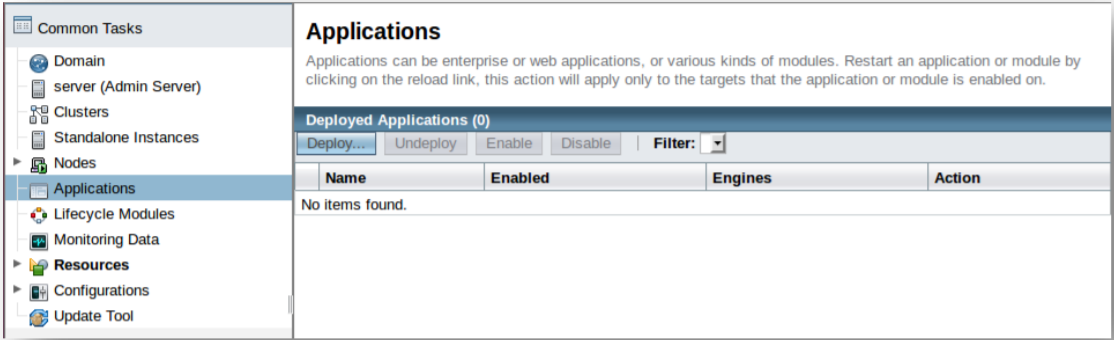
\includegraphics[width=\textwidth]{C5_InSer1}

A continuación hay que hacer \textit{click} sobre el botón \textit{Deploy} e indicar la ruta en la que se encuentra el archivo \textit{.war} , después una vez que se haga \textit{click} sobre el botón OK ya estará la aplicación publicada y funcionando.

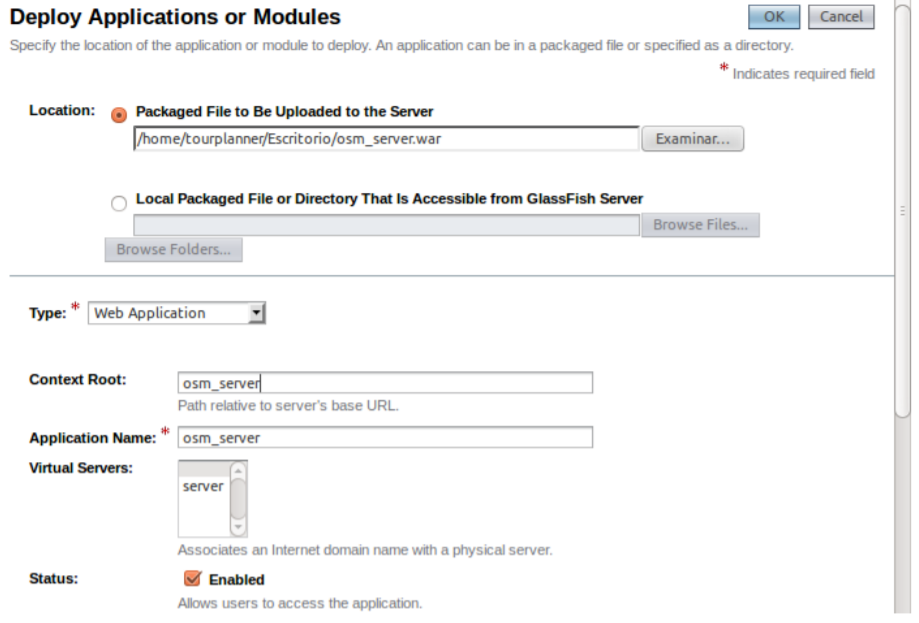
\includegraphics[width=\textwidth]{C5_InSer2}


\subsection{Instalación de la aplicación en el cliente}
Para realizar la instalación de nuestra aplicación \textit{Android} en un dispositivo físico o un emulador necesitaremos seguir los siguientes pasos:
\begin{itemize}
\item En caso de un dispositivo físico será necesario que éste se encuentre conectado al sistema en el que tengamos la aplicación.
\item Una vez tengamos lista la aplicación pulsaremos el botón de \textit{Play} en \textit{Android Studio}.

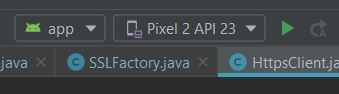
\includegraphics[width=\textwidth]{C5_installAndroid}

\item \textit{Android Studio} será el encargado de instalar el archivo \textit{.apk} dentro del dispositivo y lo ejecutará automáticamente.


\includegraphics[width=\textwidth]{C5_PlayAn}

\textbf{AC: ACTUALIZAR SEGUN MANUAL DE SUSO}
Hay que tener en cuenta que para el correcto funcionamiento de la aplicación hay que seguir correctamente los pasos de compilación explicados en el apartado \textit{Compilación del cliente}, prestando especial atención al punto en el que se establece la dirección IP y puerto del servidor.

\end{itemize}
\subsection{Ejecución de la aplicación}
Para lograr que la aplicación se ejecute correctamente sin la necesidad de contar con un servidor y un cliente independientes, se han incluido en el USB del proyecto las máquinas virtuales correspondientes a el cliente y el servidor. De esta forma podremos ejecutar la aplicación con un solo ordenador.

Cabe destacar que para lograr que ambas máquinas virtuales se comuniquen entre sí correctamente, se ha utilizado el programa \textit{LogMeIn Hamachi} que nos permite crear redes virtuales entre ambas máquinas a través de Internet.
\subsubsection{Ejecución de la aplicación servidor}
Para ejecutar la aplicación servidor, se importa la máquina virtual \textit{Servidor-Ubuntu 18.04 LTS} en \textit{VirtualBox} (hay más software de creación de máquinas virtuales pero este es el que se ha utilizado).

\textbf{AC: FOTO}

\subsubsection{Ejecución de la aplicación cliente}
Para ejecutar la aplicación cliente, al igual que con la aplicación servidor, se importa la máquina virtual \textit{Cliente-Windows 10} en \textit{VirtualBox}.

Una vez se haya iniciado la máquina virtual, se hace doble \textit{click} sobre el entorno de desarrollo \textit{Android Studio}. A continuación, hacemos doble \textit{click} sobre el icono \textit{Play}.

\textbf{AC: FOTO}

\section{Manual del usuario}





\bibliographystyle{plain}
\bibliography{bibliografiaAnexos}

\end{document}
